\documentclass[addpoints, 12pt]{exam}%, answers]
\usepackage[utf8]{inputenc}
\usepackage[T1]{fontenc}

\usepackage{lmodern}
\usepackage{arydshln}
\usepackage[margin=2cm]{geometry}

\usepackage{enumitem}

\usepackage{enumerate}
\usepackage{breqn}
\usepackage{parskip}

\usepackage{amsmath, amsthm, amsfonts, amssymb}
\usepackage{graphicx}
\usepackage{tikz}
\usetikzlibrary{arrows,calc,patterns}
\usepackage{pgfplots}
\pgfplotsset{compat=newest}
\usepackage{url}
\usepackage{multicol}
\usepackage{thmtools}

\usepackage{caption}
\usepackage{subcaption}

\usepackage{pifont}

% MATH commands
\newcommand{\bC}{\mathbb{C}}
\newcommand{\bR}{\mathbb{R}}
\newcommand{\bN}{\mathbb{N}}
\newcommand{\bZ}{\mathbb{Z}}
\newcommand{\bT}{\mathbb{T}}
\newcommand{\bD}{\mathbb{D}}

\DeclareMathOperator{\dom}{dom}


\newcommand{\spc}{\vspace*{0.5cm}}
\CorrectChoiceEmphasis{\color{red}}

\begin{document}
	\noindent \hrulefill \\
	MATH-241 Calculus I \hfill Created by Rukiyah Walker\\
	Homework 2 \hfill Spring 2023\\\vspace*{-0.7cm}
	
	\noindent\hrulefill
	
\vspace*{0.5cm}

\qformat{\rule{0.3\textwidth}{.4pt} \begin{large}{\textsc{Question}} \thequestion \end{large} \hspace*{0.2cm} \hrulefill \hspace*{0.1cm} \textbf{(\totalpoints\hspace*{0.1cm} pts)}}

\begin{questions}

\question[1]
A tangent line is:
    
\begin{choices}
\choice A line that goes through a circle.
\CorrectChoice A line that touches a curve at a single point.
\choice A line that intersects two points on a curve.
\choice A curve.
\end{choices}

\spc

\question[1]
A secant line is:

\begin{choices}
\choice A line that touches a curve at a single point. 
\choice A curve.
\CorrectChoice A line that intersects two points on a curve.
\choice The diameter of a circle.
\end{choices}

\spc

\question[1]
What is the slope of the tangent line?

\begin{choices}
\choice $y = mx + b$
\choice The secant line.
\choice The average velocity.
\CorrectChoice The limit of the slopes of the secant lines.
\end{choices}

\spc

\question[1]
What is the slope of the secant line?

\begin{choices}
\CorrectChoice The average velocity.
\choice The tangent line.
\choice The diameter of a circle.
\choice The instantaneous velocity.
\end{choices}

\spc
\newpage
\question[1]
What is the instantaneous velocity?

\begin{choices}
\choice Change in position over change in time.
\CorrectChoice The slope of the tangent line.
\choice $s(t) = 4.9t^2$
\choice Acceleration. 
\end{choices}

\spc

\question[1]
$\lim_{x \to a} f(x) = L$ means:

\begin{choices}
\choice "the limit as $x$ approaches $a$ is $f(x)$"
\choice "the limit of $f(x)$, as $x$ approaches $a$, does not exist"
\CorrectChoice "the values of $f(x)$, as $x$ approaches $a$, approaches $L$"
\choice "the limit, $L$, equals $f(x)$"
\end{choices}

\question[1]
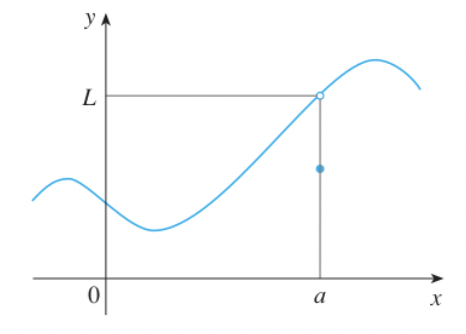
\includegraphics[width=0.4\textwidth]{241-limit case 2.png}

Which of the following represents the graph above?

\begin{choices}
\CorrectChoice $L \neq f(a)$
\choice $f(a)$ not defined.
\choice $L = f(a)$
\choice $\lim_{x \to a} f(x) = \infty$
\end{choices}

\spc

\question[1]
$\lim_{x \to a} f(x) = L$ if and only if:

\begin{choices}
\choice $\lim_{x \to a^+} f(x) = L$ and $\lim_{x \to a^-} f(x) = M$, with $L \neq M$
\CorrectChoice $\lim_{x \to a^+} f(x) = L$ and $\lim_{x \to a^-} f(x) = L$
\choice $\lim_{x \to a^+} f(x) = L$ does not exist.
\choice $\lim_{x \to a^-} f(x) = L$ does not exist.
\end{choices}

\spc

\question[1]
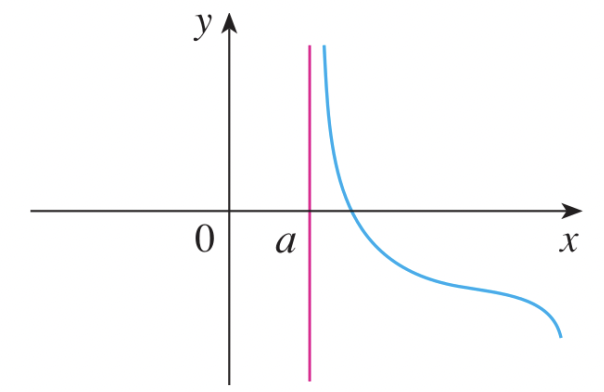
\includegraphics[width=0.4\textwidth]{241-infinite limits.png}

Which of the following represents the graph above?

\begin{choices}
\choice $\lim_{x \to a^-} f(x) = \infty$
\choice $\lim_{x \to a} f(x) = \infty$
\choice $\lim_{x \to a} f(x)$ does not exist.
\CorrectChoice $\lim_{x \to a^+} f(x) = \infty$
\end{choices}


\question[1]
Which of the following is a case when the vertical line, $x = a$, is called a vertical asymptote of the curve $y = f(x)$?

\begin{choices}
\choice When the limit does not exist. 
\choice When $x = y$
\CorrectChoice $\lim_{x \to a} f(x) = \infty$
\choice When there is a horizontal asymptote.
\end{choices}



\end{questions}

\end{document}